\section{The Space Environment}
Surrounding the Earth there exists a sparse gas of ions and electrons called a \emph{plasma}. These particles reside in a state of constant flux, resulting from a tenuous and dynamic balance of energy fluxes -- streaming in from the sun, and back and forth within the Earth's terrestrial atmosphere. Every human-made satellite has passed through it; the vast majority of satellites, with the exception of deep-space probes, live out their entire existence within it. Aside from the lunar astronauts of the Apollo era, every single human in space has spent the duration of their journey within this constantly-evolving cloud of matter. The technology ubiquitous in our day-to-day lives -- instant international communication, satellite-aided global positioning systems -- all require signals to be transmitted through it. We call this region, from say, an altitude of 100 km on out to the moon, the \emph{Space Environment}.

%The space environment is defined largely by the Earth's magnetic field. We refer to this system as the \emph{Magnetosphere}, and the plasma contained within it as the \emph{Plasmasphere}. 

\begin{figure}[t]
\begin{center}
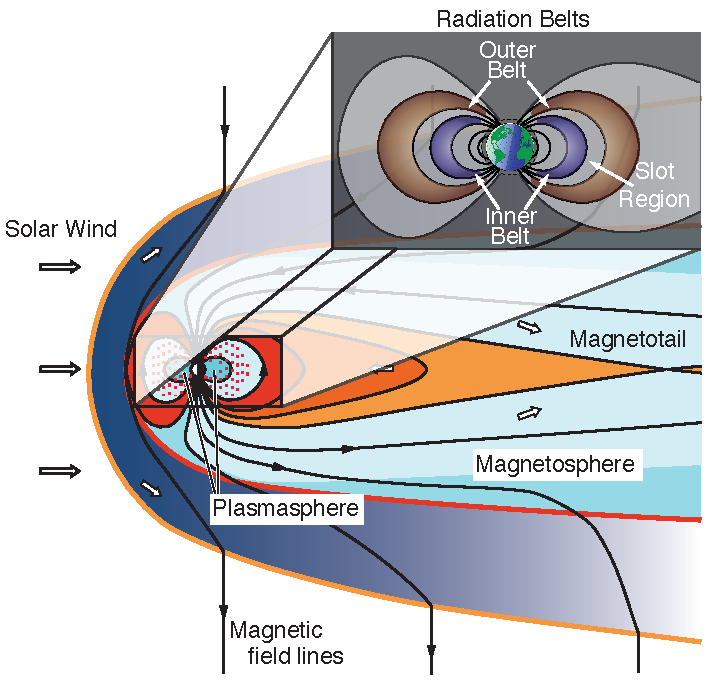
\includegraphics{figures/space_environment_figure.pdf}
\caption[Diagram of the various regions of the space environment]{The various regions of the near-Earth Space Environment. The topology of the space environment is driven by the Earth's magnetic field, and by the solar wind. The radiation belts are shown in the inset. Figure from \cite{Graf2013}.}
\label{fig:space_environment}
\end{center}
\end{figure}

The space environment is largely defined by the Earth's magnetic field, which constrains the plasma to a toroidal shape. The region in which the Earth's magnetic field impacts significant action is called the \emph{magnetosphere}, and the region of constrained plasma immediately surrounding the Earth the \emph{plasmasphere}. The majority of the particles within the plasmasphere are cold, with energies less than $\sim$ 1 eV. However, a sparse population of high-energy particles exist, with energies approaching 10 MeV, and velocities approaching the speed of light. These so-called `killer electrons', while sparse in number, present a significant hazard for both electrical systems, and to living organisms in space \citep{Barth2003}. The populations of these particles form two shells, known as the Van Allen radiation belts, separated by a depleted `slot' region. Understanding the behavior of these high-energy particles are key to sustained human activity in space. 

The population of high-energy particles is driven by a complex balance of sources, acceleration mechanisms, and loss processes. This thesis considers the effect of one such loss mechanism: the action of radio waves generated by terrestrial lightning through a resonant scattering process known as \emph{Lightning-induced Electron Precipitation} (LEP), and examines the regions of the space environment in which losses due to LEP may be substantial. We perform this study through extensive numerical simulation of single LEP events, under a variety of space weather conditions, and examine global trends by extrapolating over a global lightning activity dataset.



\section{Motivation}
\subsection{The Radiation Belts}
The Van Allen radiation belts, first measured in 1958 by \cite{VanAllen1958} on the Explorer I and III satellites, represent one of the earliest major discoveries of the American space program. The belts are an enhancement in very-high-energy particles (E $>$ 100 keV), which extend from 1.2 to 7 earth radii along the equator, and follow the Earth's magnetic field to $\sim \pm65^\circ$ latitude \citep{Walt1994}. While the location and population of the belts are highly dynamic, it is customary to divide the population of high-energy particles into two toroidal shells: an inner belt below $\sim$ 3 Earth radii; an outer belt between $\sim$ 3 and 7 Earth radii; and a `slot' depletion region between 2 and 3 Earth radii. The radiation belts are dominantly populated by electrons ($e^-$) and Hydrogen ions ($H^+$). Geomagnetically-trapped particles are confined by the Earth's magnetic field, and exhibit a helical bouncing motion, reflecting between fixed points near the northern and southern poles.

It was recognized early on that the ionizing effects of high-energy electrons represented a hazard for both humans and electronics in space. The Apollo manned spaceflight missions dealt with the risk of ionizing radiation both by incorporating additional aluminum shielding, and by designing their orbit trajectory to minimize time spent in the Van Allen belts \citep{Apollo1973}. Astronauts aboard the International Space Station wear passive dosimeters to measure total exposure; furthermore, the ISS includes radiation-safe regions which are better-shielded to the space environment, for use in cases of extreme solar or geomagnetic activity \citep{ugh}. 

As silicon gate sizes continue to shrink, electronics have become increasingly susceptible to radiation-related failures. Single-event upsets (SEU) can occur when a high-energy particle impinges on a volatile memory circuit, imparting enough energy to erroneously change a bit from 0 to 1, or 1 to 0. The effects of SEU can be mitigated through specialized design practices, including triple-redundant systems and larger gate sizes, and are regarded as `soft' failures from which a system can be designed to survive. Of additional risk are catastrophic failure events -- for instance, in which an energetic particle can impinge on the oxide layer of a FET transistor, and create an electrical short, either temporary or permanent. Such an event can render spaceborne electronics useless. Furthermore, the constant influx of charged particles can slowly degrade the doping of bulk silicon transistors, resulting in slower switching speeds and reduced gains through total-dose effects.

\subsection{Sources and Loss Processes}
The radiation belts are generally populated by the stream of particles arriving via the solar wind, which provides a steady flow of cold electrons (velocities $\sim 300$ km/sec, and temperatures $\sim 10^{-5}$ Kelvin) \citep{Montgomery1974, Tascione1988}. These particles are then gradually accelerated to relativistic energies through a variety of acceleration processes within the magnetosphere, (itself a very open research topic) such as resonant interactions with ULF waves, chorus waves, and magnetotail processes \citep{Shprits2006,  Bortnik2007a, Thorne2013}.

The dynamics of the radiation belts are marked with periodic filling events, in which the distribution of high-energy particles rapidly increase \citep{Horne2005, Baker2014}. In the absence of other interactions, these particles would remain trapped by the Earth's magnetic field, and populations would continue to increase indefinitely. However the influx of new particles is balanced by an equally-complex set of loss processes.

Throughout the 1960s and 1970s, a wealth of research was performed on the lifetime of energetic radiation belt particles, most notably through a series of atmospheric nuclear detonations known as the \emph{Starfish} project\footnotemark. Starfish was a 1.4 megaton nuclear device, detonated 400 km above Johnson Island on July 9, 1962, which provided an artificial, local enhancement to the inner radiation belt at approximately 1.2 Earth radii \citep{Hess1963}. Data from particle detectors aboard several early satellites (Telstar, Injun, Ariel, and Tracc) were then used to study the lifetimes and dispersion characteristics of energetic protons and electrons. Starfish electrons were found to be very long-lived, with lifetimes on the order of $\sim 2$ years \citep{Beall1967}. Furthermore, in the months following the Starfish detonation, seven satellites, (including Telstar 1, the first commercial communications satellite, launched one day after the Starfish detonation) experienced catastrophic failures \citep{Wenaas1978, Barth2003, Conrad2010}, inspiring a decades-long research interest in the lifetime of radiation belt particles, and anthropogenic techniques for the mitigation of nuclear-injected particles.

The earliest loss-mechanism theories considered Coulomb scattering against the nucleii of atmospheric neutral constituents \citep{Walt1964}. This model showed reasonable agreement with Starfish particles at the lowest altitudes ($\sim$ 1.1 Earth radii), but greatly overestimated particle lifetimes for the majority of inner-belt electrons, indicating that other, unaccounted-for loss processes must be present. 
\footnotetext[1]{While the Starfish detonation was the greatest yield and highest-altitude, and thus of the greatest interest in radiation belt physics, it was not by far an isolated event. Between 1955 and 1962, with a lapse following an international armistice between 1958 and 1961, the United States performed twelve atmospheric nuclear tests, at altitudes ranging from 6 to 540 kilometers, with yields in the kiloton range, reaching a maximum with Starfish at 1.4 megatons. Simultaneously, between 1961 and 1962, the Soviet Union performed five high-altitude detonations between 1.2 and 300 kilotons. An international moratorium on high-altitude detonations took place in 1963 with the High Altitude Nuclear Test Ban Treaty \citep{Hess1964b, Schwelb1964, Hoerlin1976, Norris1996}.}


\section{Previous Work}
% PUT IN AN ASIDE ABOUT LIGHTNING AND VLF HERE -- You'll need to talk about the guided portion, etc etc

\subsection{Wave-Particle Interactions}
Recognizing the need for additional loss mechanisms, It was soon theorized that resonant interactions with radio waves could significantly alter the reflection height of trapped particles, and in turn drive these particles further into the neutral atmosphere, where they stood a much higher chance of colliding with neutral constituents, and eventually precipitating into the neutral atmosphere. Unlike in free space, the charged medium of the plasmasphere allows propagation of only certain frequencies and modes of radio wave (see section \ref{section:waves_in_plasmas}). Right-hand, circularly-polarized waves in the VLF band ($\sim < 30 $ kHz) are common in the plasmasphere, and arise from a variety of generation mechanisms. These waves are known as \emph{whistlers}, named for the descending, whistle-like tones originating from distant, broadband impulses. Terrestrial lightning is a persistent source of whistlers, with $\sim$ 50 flashes/sec occurring globally; each whistler can propagate through the magnetosphere and persist for several seconds. Within literature, whistler waves are often divided into two categories: ``ducted'' waves, which propagate in temporary, waveguide-like enhancements in plasma density, with wavenormal vectors nearly parallel to the background magnetic field, and ``magnetospherically reflecting'' (MR) whistlers, which are not constrained to a duct, and generally have a much more-oblique wavenormal angle. Figure \ref{fig:whistlers} shows an example of a whistler wave and its causative lightning stroke. 
Whistler waves can also be generated naturally within the plasmasphere (\emph{chorus} and \emph{hiss}) or be induced via high energy, ground-based VLF transmitters \citep{Graf2013}. (It should be noted that whistlers are not the only category of waves relevant to the radiation belts -- see the review paper by \cite{Thorne2010a} for an overview of various other waves).

\begin{figure}[t]
\begin{center}
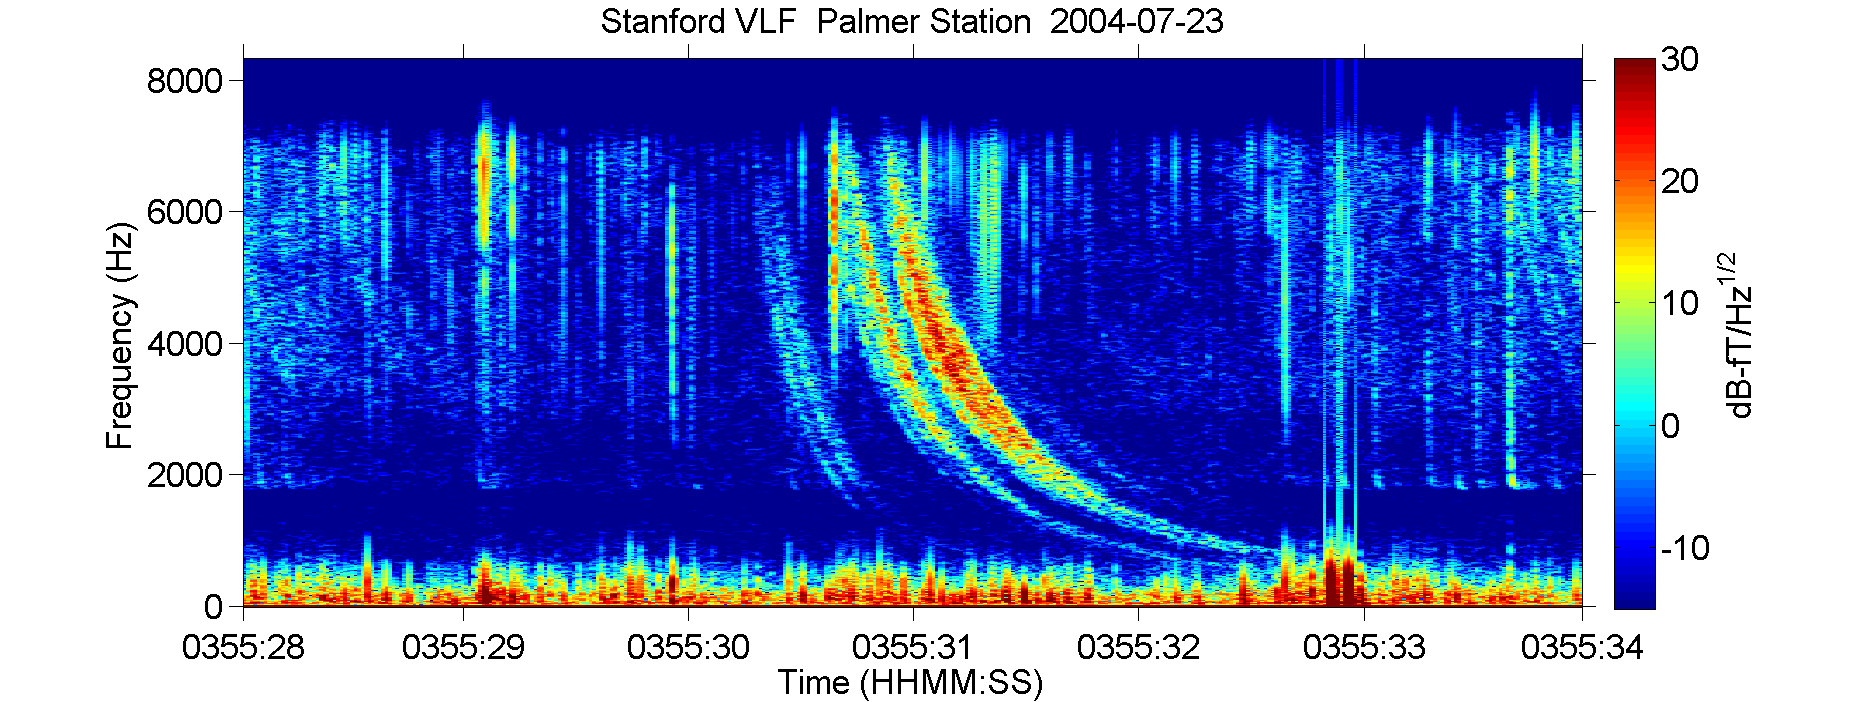
\includegraphics[width=0.95\textwidth]{figures/Whistler_radio_palmer_2004-07-23_T035528.png}

\caption[An example of a lightning-generated whistler wave]{Time-frequency spectrogram of VLF radio wave data from Palmer Station, Antarctica. The short-duration vertical impulses are \emph{'sferics}: broadband radio noise radiating directly from a lightning discharge. The curved, sweeping tones result from a fraction of the radio energy propagating out into the plasmasphere, reflecting at the northern hemisphere, and returning to the southern hemisphere. The plasmasphere is a dispersive medium; lower frequencies propagate at a slower velocity than higher frequencies, resulting in the transformation of an impulsive ``click'' into a descending whistling tone. Figure by Dr. Dan Golden.\footnotemark[2] }
\label{fig:whistlers}
\end{center}
\end{figure}

The concept of lightning as a loss mechanism for radiation belt electrons was first proposed by \cite{Dungey1963}, and subsequently by \cite{Cornwall1964}, through resonant interactions with whistler waves. \citeauthor{Dungey1963} provided order-of-magnitude estimates for electron lifetimes, arguing for the significance of LEP in the inner radiation belt, and against for the outer radiation belt, and proposed an anthropogenic source of whistlers as a provisional loss mechanism in the event of further nuclear enhancements. 

Shortly thereafter, \cite{Kennel1966b}, and subsequently \cite{Lyons1973}, provided an alternative mathematical framework for the diffusion of radiation belt particles due to random-walk interactions with incoherent whistler mode waves known as \emph{plasmaspheric hiss}. From here, studies of wave-induced precipitation mechanisms can be grouped into two categories: coherent studies (the ``Liouville" approach), in which known particles are subjected to a known wave event, and incoherent studies (the ``Fokker-Planck'' approach), in which distributions of particles evolve through repeated, stochastic interactions with broadband radio wave activity.

\footnotetext[2]{Available through Creative Commons at \emph{https://en.wikipedia.org/wiki/Whistler\_(radio)}}

\subsection{LEP measurements}
The first one-to-one measurements of precipitating electrons associated with causative whistlers were presented by \cite{Voss1984}, and subsequently analyzed in \cite{Voss1998}, confirming the feasibility of LEP as a radiation belt loss mechanism. However, due to the sporadic nature of LEP and the dearth of space vehicles to measure it, \emph{in-situ}, one-to-one measurements of LEP remain somewhat rare.
Fortunately LEP can be measured terrestrially across a great distance by examining the perturbations to VLF-band transmitter signals as they propagate in the waveguide formed by the Earth and the charged ionosphere. Additional charges imparted by LEP to the ionosphere can perturb this waveguide, and in turn affect the measured amplitude and phase of transmitted signals. These sporadic events (frequently known as ``Trimpi" events, a nod to their discovery by Mike Trimpi in \cite{Trimpi1973}), have been studied for several decades \citep{Trimpi1973, Carpenter1984, Inan1988, Burgess1993}. These works further confirm the existence and frequency of LEP events; however due to the nature of the waveguide sensing method, it is difficult to obtain direct electron flux estimates without substantial modeling.
Evidence for the seasonal variation of LEP is shown in \cite{Gemelos2009}, who present correlations between lightning over the continental United States and particle flux measurements from the DEMETER spacecraft at $\sim$ 600 km.

\subsection{Modeling of single LEP events}
A substantial history of numerical modeling of LEP exists at Stanford, beginning with the thesis work of \cite{Inan1977}, who performed numerical simulations of pitch-angle scattering due to short-duration, monochromatic, ducted whistler waves. This work was then elaborated on throughout the 1980s in a series of test-particle simulations \citep{Inan1982, Chang1983, Chang1983b, Chang1985, Inan1989}, which directly simulate the effect of whistler waves on discrete collections of electrons in the time domain.

Gyrorotation-averaged equations of motion for the interaction of waves and trapped particles were derived by \cite{Bell1984}. Combined with the derivations of \cite{Ristic1992}, the thesis work of \cite{Ristic1993} and subsequently \cite{Ristic1998} provided a mathematical framework for the interaction of generic whistler waves and trapped particles, and demonstrated the relative importance of oblique wave interactions. 

The thesis work and subsequent publications of \citeauthor{Lauben1998} \citep{Lauben1998, Lauben1999, Lauben2001} represented a full numerical treatment of precipitation due to a single lightning stroke, combining test-particle simulations with a numerical raytracing scheme to estimate whistler wave intensity vs. location, frequency and time. The thesis work of \cite{Bortnik2005} brought further detail to the simulation of LEP, again using a raytracing scheme, and incorporating, among other improvements, Landau damping calculations and multiple resonant modes. The work of \citeauthor{Lauben1998} and \citeauthor{Bortnik2005} primarily differ in their treatment of the resonant interaction: \citeauthor{Lauben1998} uses a test-particle approach to track the change in particle pitch angles across long distances; \citeauthor{Bortnik2005} uses a hybrid coherent / incoherent scatter model, in which the coherent interactions are computed for a collection of particles along a field line with a monochromatic frequency wave, and are then considered independent from other locations and wave frequencies; the resulting resonant interactions are then summed in quadrature across all frequencies and latitudes, to provide a pseudo-coherent, RMS scattering approximation.

The wave-particle interaction model of \cite{Bortnik2005, Bortnik2006} was then applied to lightning-driven precipitation through transmitter remote sensing by \cite{Peter2007}, and to narrowband, transmitter-generated waves by \cite{Kulkarni2009} to examine the efficiency of spaceborne VLF transmitters as a remediation tool for radiation belt electrons;. \cite{Cotts2011} further expanded on the \citeauthor{Bortnik2005} model by incorporating the effects of atmospheric backscatter.

The work presented in this thesis is based off of the original model from \cite{Bortnik2005}; however we provide several model improvements, including an elaborated treatment of the background plasma; a more-accurate model of variation along the longitudinal axis; and various practical code improvements.

% inan 1878, chang + inan thru the 80s, Ristic 1993, Lauben 1998, Bortnik 2005, the ABS stuff, etc
% Should we talk about incoherent methods? They're not really relevant here, but...
\subsection{Behavior of whistler waves in the magnetosphere}
Fully understanding LEP requires study of both the interaction of particles and waves, as well as the behavior of the waves and particles before and after the interaction. The LEP process spans multiple regions of the space environment, and includes physics on timescales ranging from microseconds to minutes. The behavior of whistler waves in the magnetosphere have been studied extensively using the Hamiltonian ray tracing formulation \citep{Stix1992, Landau1975}, beginning with \cite{Haselgrove1955} via a graphical construction technique, and subsequently by \cite{Haselgrove1960} via numerical computation. Over the following decades, the formulation of \citeauthor{Haselgrove1955} was applied extensively to whistler waves \citep{Kimura1966, Edgar1972}, using the `Stanford Ray Tracing Program', a FORTRAN code originally developed by \cite{Walter1969}, with significant improvements by \cite{Inan1977b, Ngo1989}, and others. In this thesis we use a modern reworking of the Stanford program, designed by Dr. Forrest Foust in \cite{Golden2010}. Despite a decades-long legacy of work, whistler ray tracing remains an active research pursuit, driven by further improvements to plasmasphere models and increased computational resources. The \citeauthor{Golden2010} model was most-recently expanded by \cite{Maxworth2017} to include warm plasma corrections.

The previously-discussed ray tracing formulations compute wave propagation paths only; a separate treatment is required to compute energy losses due to interactions with the background medium, in a process known as Landau damping. Landau damping was first applied to the whistler mode by \cite{Kennel1966}, and subsequently generalized by \cite{Brinca1972}. While the derivation is detailed, applications of the of \citeauthor{Brinca1972} equations are heavily dependent on the temperature profile used \citep{Thorne1994, Bell2002}. Within this work we use a modified temperature profile from \cite{Golden2010}, which combines results from \cite{Bell2002} and \cite{Bortnik2007}.

\subsection{Electron lifetime estimates due to LEP}
LEP is only one of numerous radiation belt loss processes; when combined with an equally dynamic and complicated set of source and loss processes, direct measurements of lifetimes due to LEP are all but impossible. As such, research on the relative contributions of each loss process to the overall timescale of radiation belt lifetimes rely heavily on approximations and models. \cite{Abel1998} divide the VLF spectrum into three separate categories -- hiss, lightning-generated whistlers, and manmade VLF transmitter signals -- and perform a diffusive calculation for each. \citeauthor{Abel1998} conclude that lightning-generated whistlers are an important second-order loss process, but that electron lifetimes are more-likely controlled by plasmaspheric hiss.

Using models of precipitation and a dataset of Trimpi events, \cite{Rodger2003} and subsequently \cite{Rodger2010} estimated the lifetime of radiation belt electrons subject to LEP losses to be on the order of 10 to 100 days, and surmised LEP may be a significant loss mechanism for the inner radiation belt. \cite{Shprits2005} assumed a constant lifetime of $\sim$ 10 days within the plasmasphere, and a faster, empirical fit outside the plasmasphere. \cite{Meredith2007}, using wave data from the CRRES spacecraft and the PADIE Fokker-Planck diffusion code, performed a comparative study of ducted whistlers, MR whistlers, and plasmaspheric hiss, for energies between 100 keV and 5 MeV, resulting in widely varying lifetimes between 1 and 10000 days, depending on energy and location. In nearly every scenario considered, \citeauthor{Meredith2007} found the effect of lightning-generated whistlers to be outweighed by hiss. However, the interaction of a short-duration whistler may not be fully captured by a diffusive code, which relies on multiple incoherent interactions to evolve a distribution of particles. \cite{barker2005} assumed lifetimes ranging from 6 to 29 days in the outer belt; \cite{Horne2005} determined outer belt lifetimes to be $\sim$ 1 day due to electron microbursts.


%\cite{Shprits2005}, using wave data from the CRRESS spacecraft and a Fokker-Planck diffusion code, estimate electron lifetimes to be on the order of 10 days, dependent on location and solar activity. 

% Abel and Thorne
% Meredeth
% Craig Rodger 2003
% 

\section{Scientific Contribution}
A lack of continuous measurements, both remote and \emph{in-situ}, combined with a wide range of electron energies, the dynamic and sporadic nature of the space environment, and the noise introduced by numerous source and loss processes, has resulted in a lack of consensus on the importance of LEP as a radiation belt loss mechanism. Within this work we seek to quantitatively determine the regions in space and energy where LEP may be of importance, using a combination of raytracing, coherent-interaction modeling, and the introduction of realistic lightning data as measured by the GLD360 lightning detection network. Through modeling, we can examine the impact of LEP independent of the added contributions of numerous other source and loss processes which may overshadow LEP.

The contributions of this work to the scientific community are:
\begin{enumerate}
\item A quantitative estimate of the persistent VLF whistler-mode energy within the plasmasphere and magnetosphere resulting from realistic measurements of terrestrial lightning activity, accounting for variation between day and night, and for variation with K$_p$.

\item Development of a novel interpolation scheme to map unstructured data from a family of rays to their corresponding grid coordinates within the magnetosphere.

\item An improved model of the longitudinal variation of LEP, and an examination of the errors introduced by a two-dimensional approximate scaling function.

\item An examination of the precipitating energy spectrum and total energy deposition below 100 km altitude resulting from LEP, as a function of geographic location, K$_p$, and time of year.

\item Determination of average lifetime estimates for radiation belt electrons subjected to LEP losses, across a wide range of energies (10 eV - 10 MeV), and L-shells (1.2 - 7).

\item Development of onboard firmware for a CubeSat-based instrumentation suite, designed for direct, \emph{in situ} measurements of LEP.
\end{enumerate}
\section{Thesis Organization}
This thesis is divided into the following chapters:
\begin{itemize}
\item Chapter \ref{chapter:physics} describes the background physics of the LEP process, the numerical methods used within this study, and the mathematical models of the various environments which we examine. 
\item Chapter \ref{chapter:power} presents a study of the persistent VLF radio energy within the magnetosphere, resulting from terrestrial cloud-to-ground lightning discharges as measured by the GLD360 dataset. Variation is explored with respect to geomagnetic longitude and K$_p$. 
%\item Chapter \ref{chapter:3dWIPP} provides a simulation of electron precipitation resulting from a canonical cloud-to-ground lightning discharge, and a discussion of various model improvements, notably with our treatment of the longitudinal axis. 
\item Chapter \ref{chapter:global_estimates} provides a simulation of electron precipitation resulting from single cloud-to-ground lightning discharges, over an array of latitudes, longitudes, and environmental conditions. Using these simulations, we then compute seasonal estimates of the global impact of LEP, driven by the GLD360 dataset. Finally we estimate the average lifetime of radiation belt electrons across a wide range of energies, by simulating electron losses from a uniform population.

\item Chapter \ref{chapter:VPM}, admittedly a bit of a tangent, presents the design of a CubeSat-based instrumentation suite, designed for direct, \emph{in-situ} measurements of LEP by taking time-and-space-coincident measurements of electron loss cone distributions, and incident VLF waves. The design provides some interesting on-board signal processing to reduce the data bandwidth significantly, and is implemented entirely in fixed-point logic using an FPGA (and \emph{no} onboard CPU). I worked on this design in the earlier years of my time at Stanford; at time of writing it is due to be launched in early 2019.
\end{itemize}

